\section{Analysis of the Problem}
\subsection{Clarification}
Based on the ten smart growth principles in `The Smart Growth Network'\cite{pdf:smart-growth}, a  smart growth metric is to be set up which can well measure how successfully a city develops.
With two mid-sized cities on two different continents selected, the problem including the following requirements can be solved:

\subsection{Requirement}
\begin{enumerate}
  \item Using the metric above, judge whether the current growth plan of each city obeys the `smart growth principles', and measure how successfully each city grows.
  \item Based on the geography, economic opportunities and prospective, work out a growth plan for each city under the smart metric, and sequence every factor in the order of potential.
  \item Revise the growth plan in \textbf{2}, given that the population changed by 50\% till 2050.
\end{enumerate}

%-------------------------------------%
%-------------------------------------%
%-------------------------------------%

\section{Introduction}
Since different cities' compositions in detail (including transportation network, residents working habits) are quite different, in order to obtain a relatively universal metric standard for city development, we need to simplify actual cities into models properly.
In this paper, our method is to divide the city into multiple (2000 \~{} 3000) square units and define their types and development levels.\\

In Athens Charter\footfullcite{conf:The-Athens-Charter}, it argues that city should be arranged according to its residential, working and recreational function.
Based on that, we define each square unit's type as one of the followings:
\begin{itemize}
  \item Residential area
  \item Working area
  \item Recreation area
  \item Open space
  \item Undeveloped area
\end{itemize}

Just to be clear, in our definition, working area contains all service facilities for residents' daily life, such as office buildings and gas stations.
Recreation area contains facilities that provide mentally enjoyment for residents, such as restrauts, libraries and parks.
Open space refers to open landscapes, including farmlands.
Undeveloped area refers to areas that can be developed in the future.\\

According to our interpretation on the ten smart growth principles \cite{pdf:smart-growth}, we merge 10 principles into 4 judging standards.
\begin{enumerate}
  \item \textbf{Mix Land Use}\\
  This standard contains the 1st, 4th and 5th smart growth principles (We denote them as Pr.1, Pr.2 and Pr.5, and we will use similar denotations in the following passage). The reason for using it is that `mix land use' facilitate residents' travelling and working, and improve communities' cultural attractions at the same time.
  \item \textbf{Open Space and Landscape}\\
  This standard contains Pr.2 and Pr.6. According to our interpretation, one of compact building design's most important goal is to provide residents with large open space to imporve their feeling of comfort. Natural protection in Pr.6 also has a tight connection with a city's open space and natural landscape.
  \item \textbf{Housing Choice}\\
  This is standard refers to Pr.3. We need to provide different people with houses accordant with their income, which means there should be residential areas around each working area with a close development.
  \item \textbf{Transportation Convenience}\\
  This standard refers to Pr.8. To provide residents with more transportation choices, we must improve public transportation system. To measure transportation convenience, we mainly consider public transportation and its convenience.
\end{enumerate}

As for Pr.7, Pr.9 and Pr.10. Since they are not easy to be quantified, we shall consider them when we make growth plans for cities, rather than set them as different metric.

%-------------------------------------%
%-------------------------------------%
%-------------------------------------%

\section{Assumptions}
\begin{itemize}
  \item \textbf{The side of each square unit measures $a = 300$ meters.}
  \item \textbf{Buildings in the same square unit has the same type and development.} Since the side length of a square unit is relatively short, the approximation is rational.
  \item \textbf{Except undeveloped areas, the development value in each square unit is a positive integer, generally no more than 3.}
  \item \textbf{Specifically, the development value in undeveloped area is zero.}
  \item \textbf{Averagely speaking, 10\% of all square units are open space.}
  \item \textbf{People in working areas and residential areas with the same development value are under the same financial condition.}
  \item \textbf{Each working area supports the same amout of people.}
  \item \textbf{Only undeveloped area and open space area with 1 development can be developed or redeveloped.}
\end{itemize}

%-------------------------------------%
%-------------------------------------%
%-------------------------------------%

\section{Setting up the model}
\begin{table}[h]
\centering
  \begin{tabular}{cc}
    \hline
    Symbol & Meaning \\
    \hline
    $A_{ij}$ & A specific square unit \\
    $T_{ij}$ & The type of area $ A_{ij} $\\
    $d_{ij}$ & The development level of area $ A_{ij} $\\
    $\lambda_{ij}$ & How much $ A_{st} $ contributes to the mix-land-use level of $ A_{ij} $ \\
    $\theta (T_{st})$ & The importance of $T_{st}$ to residents\\
    $G_m$ & Mix-land-use score\\
    $G_b$ & Beauty Score\\
    $G_h$ & Housing Score\\
    \hline
  \end{tabular}
  \caption{Symbols}
  \label{tab:symbols}
\end{table}
We record all square units in a plane coordinate system, which means every square unit can be represented as $ A_{ij}. $
Hereafter every $ A_{ij} $ represents a square unit.
Meanwhile, we use $ T_{ij} $ to represent the type of area $ A_{ij} $ and $ d_{ij} $ to represent the development level of area $ A_{ij} $.\\

\emph{In the following formulas, undeveloped areas are out of consideration. We will mention undeveloped area in the growth plan part.}\\

\subsection{Formula 1}
First of all, we consider how to measure the level of mix land use.
Since Pr.4 encourages to create walkable neighborhoods, we mainly consider working areas and recreation areas within a walkable distance from a residential area.\\

As for a specific square unit $ A_{ij} $, we consider other square units $ A_{st}$ that satisfy $$ |s-i| \leq 2, |t-j| \leq 2. $$
In this case, residents only need to walk at most $$ 3 \sqrt{2} a \approx 1.3km $$ to reach their desired square unit.
So we define its mix-metric as $$ m(i,j) = \sum_{|s-i| \leq 2, |t-j| \leq 2} \lambda_{ij}(s,t), $$ where $ \lambda_{ij}(s,t) $ represents how much $ A_{st} $ contributes to the mix-land-use level of $ A_{ij} $.\\

It's easy to note that the higher the development level of $ A_{st} $ is and the closer $ A_{st} $ is to $ A_{ij} $, the higher the mix-metric score of $ A_{ij} $ is.
However, the two different types of areas contribute differently to mix-land-use level.
To general residents, working areas are of more importance.\\

So in mix-metric, we suppose $$ \lambda_{ij}(s,t) = \frac{d_{ij} \cdot \theta (T_{ij})}{(s-i)^2 + (t-j)^2 + 1}, $$ where $ \theta (T_{st}) $ represents the importance of different area types to residents. Details are in table \ref{tab:formula-1}.\\
\begin{table}[t]
\centering
  \begin{tabular}{c|cccc}
    \hline
    $ T_{st} $ & residential area & working area & recreation area & open space \\
    \hline
    $ \theta (T_{st}) $ & 0 & 0.6 & 0.4 & 0 \\
    \hline
  \end{tabular}
  \caption{$ \theta (T_{st}) - T_{st} $ relationship}
  \label{tab:formula-1}
\end{table}

The city's mix-metric is decided by all residential areas' weighted average mix-metric $$ M=\frac{\sum_{T_{ij}=residential} \sqrt{d_{ij}} \cdot m(i,j)}{\sum_{T_{ij}=residential} 1}. $$
We use weighted means, because the higher residential area's development level is, the more mixed the city is, but not as prominent as working areas.\\

Next we present a hundred-mark system to obtain a score.
We define an adjust function $ f_{r,k} $ : $$ f_{r,k}(x) = \frac{100rx+k}{rx+k}. $$ $ f_{r,k} $ satisfies that when $x$ tends to infinity, its value tends to 100.\\

We now set the value of parameters $r$ and $k$.
According to assumption, most areas' development level do not exceed 3, so we suppose when all areas' development level is 1, the city scores 60 and when all areas' development level is 2, the city scores 85.\\

So, when all areas' development level equals to 1, the city's mix-land-use score is expected to be $$ M=\sum_{|s|\leq 2, |t|\leq 2, s^2+t^2 \neq 0} \frac{1}{s^2+t^2+1} \times \sqrt{1} \times 0.3 \approx 1.7733. $$
When all areas' development level equals to 2, the expectation is $$ M=\sum_{|s|\leq 2, |t|\leq 2, s^2+t^2 \neq 0} \frac{2}{s^2+t^2+1} \times \sqrt{2} \times 0.3 \approx 5.0157. $$
Thus we have $ r_m $ and $ k_m $ in table \ref{tab:f1-data}.\\
\begin{table}[t]
\centering
  \begin{tabular}{c|cc}
    \hline
    Parameter & $r_m$ & $k_m$ \\
    \hline
    Value & 5.8101 & -352.13 \\
    \hline
  \end{tabular}
  \caption{$r_m$ and $k_m$}
  \label{tab:f1-data}
\end{table}

So the city's mix-land-use score is $$ G_m=\frac{581.01M-352.13}{5.8101M+1}. $$\\

\subsection{Formula 2}
Secondly, we measure a city's sight and landscape.
Awaring that in city, natural landscape's main affect is to improve quality of life in the neighborhood areas, so as for any non-open-space square unit, the affect on it by landscape is $$ b(i,j) = \sum_{|s-i|\leq 2, |t-j|\leq 2, T_{st}=open} \frac{d_{st}}{(s-i)^2+(t-j)^2+1}. $$
(As previously obtained $$ \lambda_{ij}(s,t) = \frac{d_{ij} \cdot \theta (T_{ij})}{(s-i)^2 + (t-j)^2 + 1}, $$ the metric is positive correlated with the open space's development level, and negative corellated with the distance between them)\\

So the city's beauty-metric is the average of all square units, i.e. $$ B=\frac{\sum_{T_{ij}\neq open} b(i,j)}{\sum_{T_{ij}\neq open} 1}. $$\\

We define another adjust function $ f_{r,k} $ as above.
Similarly, we define when all areas' development level is 1, the city's beauty is expected to be 60, and when all areas' development level reaches 2, the expectation is 85.\\

So, when all areas' development level equals to 1, the city's mix-land-use score is expected to be $$ M=\sum_{|s|\leq 2, |t|\leq 2, s^2+t^2 \neq 0} \frac{1}{s^2+t^2+1} \times 1 \times 0.1 \approx 0.5911. $$
When all areas' development level equals to 2, the expectation is $$ M=\sum_{|s|\leq 2, |t|\leq 2, s^2+t^2 \neq 0} \frac{1}{s^2+t^2+1} \times 2 \times 0.1 \approx 1.1822. $$\\

Thus we have $ r_b $ and $ k_b $ in table \ref{tab:f2-data}.\\
\begin{table}[t]
\centering
  \begin{tabular}{c|cc}
    \hline
    Parameter & $r_b$ & $k_b$ \\
    \hline
    Value & -4.2293 & 160 \\
    \hline
  \end{tabular}
  \caption{$r_b$ and $k_b$}
  \label{tab:f2-data}
\end{table}

So the city's beauty score is $$ G_b=\frac{422.93B-160}{4.2293B-1}. $$\\

\subsection{Formula 3}
Now, we consider how to measure a city's housing choice.
Particularly, consider a person in a working area, he needs to choose a residential area around it (As above, we consider the same range of 5*5 areas) with a similar cost level, i.e. a residential area with a similar development level.
As for a specific working area $ A_{ij} $, the housing-metric for people working there is $$ h(i,j) = 1 - \frac{min(d_{ij}, min_{|s-i|\leq 2, |t-j|\leq 2, T_{st}=residential} |d_{st} - d_{ij}|)}{d_{ij}}. $$
Since development level is a positive integer no more than 4, so housing-metric's value is limited.
Thus we don't use adjust function $ f_{r,k} $, but directly define the area's housing score $$ G_h = 100 \times \frac{\sum_{T_{ij}=work} h(i,j)}{\sum_{T_{ij}=work} 1}. $$\\

Note that we don't define the city's housing score as the average of all working areas' housing scores, but by all people working in the area(the higher the development is, the more people are working there).
According to our assumption, we simply suppose all people in a working area are well-distributed.\\

\subsection{Formula 4}
Generally speaking, changing lines in a city's public transportation system is relatively easy.
So when we consider a city's transportation-metric, we only consider whether there exists a bus station in a square unit.
If in a square unit's neighborhood (in this case, 3*3 neighborhood) there exists a bus station, we say the square unit is convenient.
The transportation score is then defined as $$ \frac{\#\left\{(i,j)|(i,j) \ is \ convenient\ and \ not\  unused\right\}}{\#\left\{(i,j)|(i,j) \ is \ not \ unused\right\}} * 100. $$\\

In the following evaluation, we calculate the average score of the four scores above as the city's overall score.
But it is neccessary to mention that this overall score only roughly represents whether this city follows all smart growth principles.
Since the four scores are not concordant, we should take more notice of the four scores separately to evaluate a city's growth and its focus points.\\

%-------------------------------------%
%-------------------------------------%
%-------------------------------------%

\section{The two mid-sized cities}
\subsection{Gernal information}
We choose \textbf{Nottingham} in Great British and \textbf{Barrie} in Canada as our target cities.
To simplify the functional distribution, we divide the two cities into square units (300m $\times$ 300m).
With the help of Google map and OpenStreetMap, the following data is collected:
\begin{itemize}
  \item Functional type of the block
  \item Development level (between 1 and 3)
  \item Bus stop number (or other public transport station)
\end{itemize}
To put it simple, we have the following figure \ref{fig:subfigure:barrie-development}, \ref{fig:subfigure:barrie-bus}, \ref{fig:subfigure:nottingham-development}, \ref{fig:subfigure:nottingham-bus} showing the distribution.
\begin{figure}[htb]
  \label{fig:two-cities}
  \centering
  \subfigure[Barrie development]{
    \label{fig:subfigure:barrie-development}
    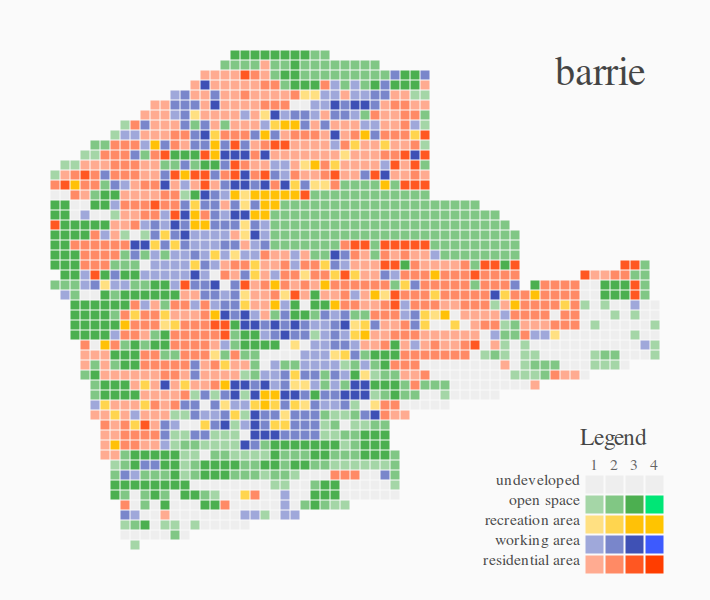
\includegraphics[width=7.5cm]{pic/barrie-development.png}
  }
  \subfigure[Barrie bus station]{
    \label{fig:subfigure:barrie-bus}
    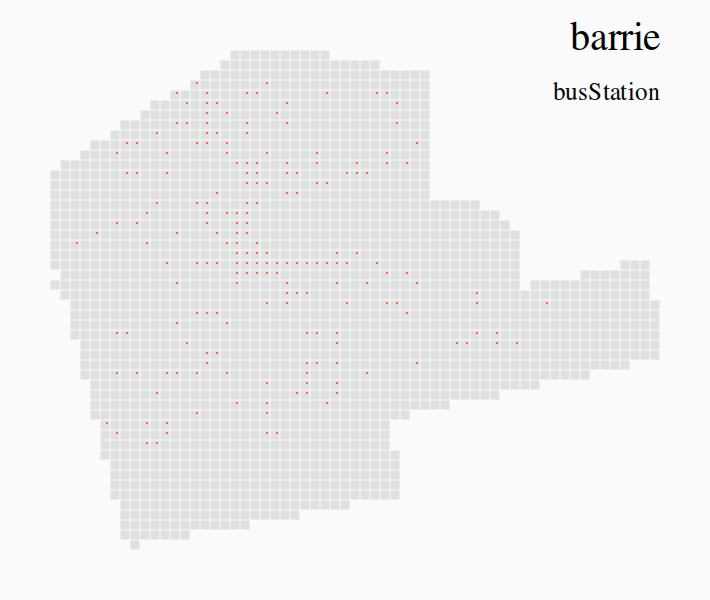
\includegraphics[width=7.5cm]{pic/barrie-busStation.png}
  }
  \subfigure[Nottingham development]{
    \label{fig:subfigure:nottingham-development}
    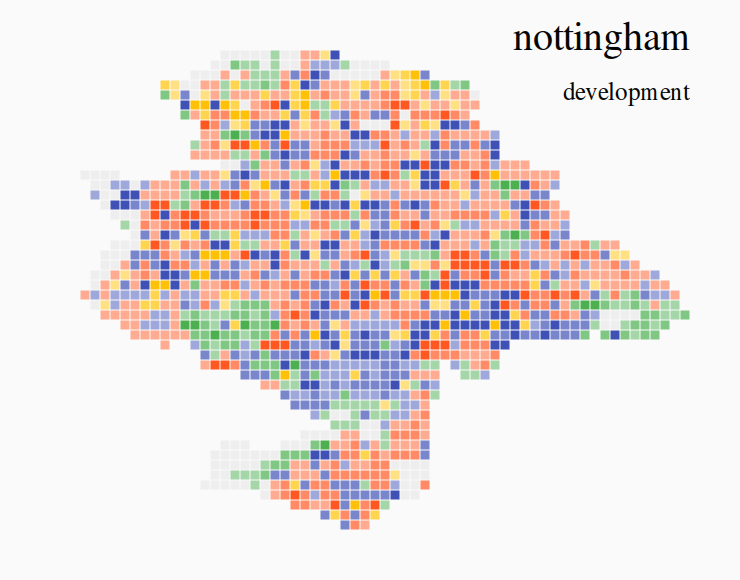
\includegraphics[width=7.5cm]{pic/nottingham-development.png}
  }
  \subfigure[Nottingham bus station]{
    \label{fig:subfigure:nottingham-bus}
    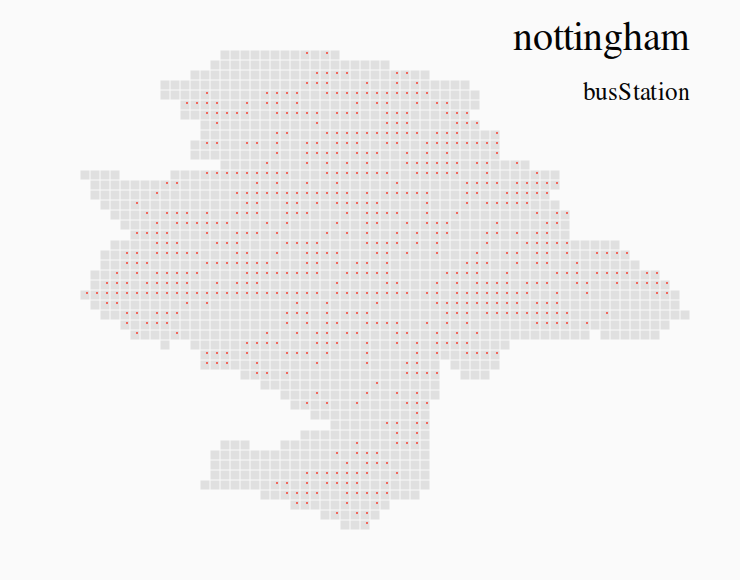
\includegraphics[width=7.5cm]{pic/nottingham-busStation.png}
  }
  \caption{}
\end{figure}

\subsection{Analysis of Nottingham}
\begin{table}[t]
\centering
  \begin{tabular}{c|cccc}
    \hline
    Type & residential area & working area & recreation area & open space \\
    \hline
    Accounting for & 49.30\% & 32.07\% & 10.25\% & 13.96\% \\
    \hline
    Average level & 1.59 & 1.96 & 1.85 & 1.53 \\
    Average level* & 1.66 & 2.28 & 2.05 & 1.53 \\
    \hline
  \end{tabular}
  \caption{Notthingham Distribution Data\footfullcite{pdf:the-nottingham-growth-plan}}
  \label{tab:nottingham-data}
\end{table}

As is shown in figure \ref{fig:subfigure:nottingham-development} \ref{fig:subfigure:nottingham-bus} and in table \ref{tab:nottingham-data}, the urban area of Nottingham city mainly consists of residential area, while open space accounts little. (Note: * means `Under government's plan')
It is worth noticing that working and recreational area has a relatively high development level, which is closely related to Nottingham's paying attention to technology, retail trade and advanced education.
However, it means that residential area has a lower development comparing to working area, indicating that the government's focus has long been on economic growth rather than people's happiness.\\
\begin{table}[t]
\centering
  \begin{tabular}{c|cccc|c}
    \hline
    Item & mix land use & beauty & residential choice & transport convenience & average \\
    \hline
    Score & 70.60 & 72.20 & 86.91 & 93.41 & 80.78 \\
    Score* & 75.14 & 73.33 & 84.51 & 92.30 & 81.32 \\
    \hline
  \end{tabular}
  \caption{Notthingham Score under Smart Growth Metric}
  \label{tab:nottingham-score}
\end{table}

Combining data from table \ref{tab:nottingham-score} and distribution in figure \ref{fig:subfigure:nottingham-development} \ref{fig:subfigure:nottingham-bus}, we can find that working area contentrates in the middle part of the city's downtown, while residential and recreation area scatters around the downtown, which leads to a decrease in the score of mix land use. (Note: * means `Under government's plan')
As for the low performance in beauty, it seems contradictory to the temperate maritime climate, which is very suitable for plants to grow.\\

Nevertheless, if considering that Nottingham has a far more prosperous economy than the rest of Britain\footfullcite{wiki:nottingham-gdp}, it is not surprising that Notthingham, known as `a Technology City', inevitably sacrifices open space to give way to economic and technology development.
The low beauty score is against Pr.6, which emphasizes `critical environmental areas';
the convenient transport and diverse choices in residential area matches Pr.3 \& Pr.8.\\

\begin{figure}[htb]
  \label{fig:nottingham-patch-diff}
  \centering
  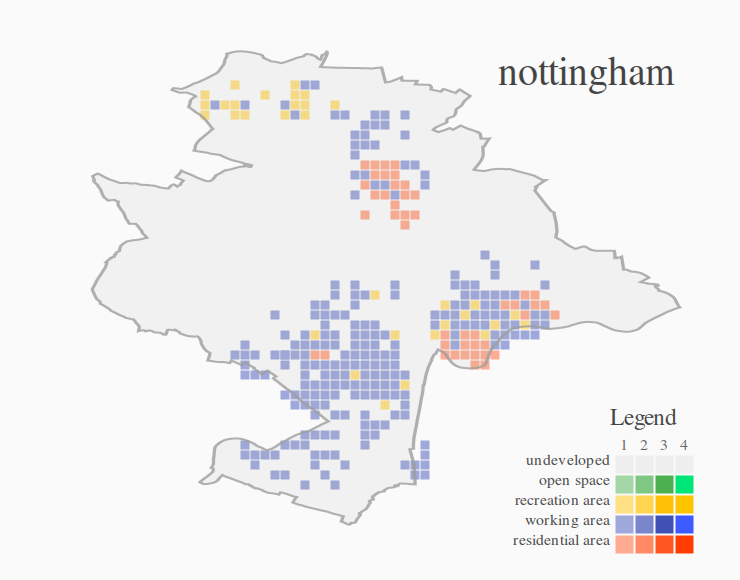
\includegraphics[width=7.5cm]{pic/nottingham-patch-diff-development.png}
  \caption{Nottingham development according to the government's plan}
\end{figure}
According to the government's growth plan and our smart growth metric, the city has some improvements, which is shown in figure \ref{fig:nottingham-patch-diff}.
It can be easily found that the following areas have a greater priority in the government's plan:
\begin{itemize}
  \item working area in downtown
  \item railway station neighbourhood
  \item northern residential and recreation area
\end{itemize}
To sum up, the government still pays great attention to working area.\\

As for the updated score under the government's plan in table \ref{tab:nottingham-data} and table \ref{tab:nottingham-score}, the residential choice score decreases due to the continuing ignorance of people's housing quality.
On the other hand, there is improvement in mix land use, for the sake of the development in the two area outside downtown.\\

It is worth pointing out that, the growth plan we found doesn't refer to any development in open land; the file heavily depicts the techinal improvement for the city's landmarks - Boots and Biocity.
So it can be inferred that the government decides to further enhance the city's dominant industry.
The decision may meet its growth need to some extent, but it is still far from `Smart Growth Principle'.

\subsection{Analysis of Barrie}
\begin{table}[t]
\centering
  \begin{tabular}{c|cccc}
    \hline
    Type & residential area & working area & recreation area & open space \\
    \hline
    Accounting for & 35.3\% & 20.97\% & 15.47\% & 36.30\% \\
    \hline
    Average level & 1.66 & 1.78 & 2.08 & 2.16 \\
    \hline
  \end{tabular}
  \caption{Barrie Distribution Data}
  \label{tab:barrie-data}
\end{table}

As is shown in figure \ref{fig:subfigure:barrie-development} \ref{fig:subfigure:barrie-bus} and in table \ref{tab:barrie-data}, working and recreation area has a rather small portion, while recreation area and open space develops much better than the rest.\\

The city of Barrie can be divided into three S-shape stripe zones: the left part is mostly residential, the middle part commercial, the right part mixing residents and recreation.
The high development of recreation area should owe to various winter-sport stadiums in the right zone, which is also a feature of city Barrie.
The heavy forest and large water area around the borderline of Barrie adds to the natural environment of the city's beauty; however, the heavy occupancy of land also forms an obstacle to the commercial development.
Comparing to Nottingham's terrian (see figure \ref{fig:subfigure:nottingham-development}), Barrie has a lower density of working area at the borderline, which may interfere with commercial communication.\\
\begin{table}[t]
\centering
  \begin{tabular}{c|cccc|c}
    \hline
    Item & mix land use & beauty & residential choice & transport convenience & average \\
    \hline
    Score & 54.24 & 92.11 & 64.06 & 50.67 & 65.27 \\
    Score* & 57.93 & 92.50 & 62.73 & 57.70 & 67.72\\
    \hline
  \end{tabular}
  \caption{Barrie Score under Smart Growth Metric}
  \label{tab:barrie-score}
\end{table}

In table \ref{tab:barrie-score}, the first three scores reflects that the three `S-stipe zones' largely interrupts Barrie's adapting to `Pr.1'(mix land use) and housing choice in `Pr.3'. (Note: * means `Under government's plan')
It's worth mentioning that roads in Barrie are a lot wider (and the distribution is more discrete than in Nottingham), so people tenf to drive instead of taking a bus, which is contrary to diverse transport choices in `Pr.8'.\\

We looked up for the plan of Barrie government \cite{pdf:barrie-downtown-plan} \cite{pdf:barrie-waterfront} \cite{pdf:barrie-official-plan} \cite{pdf:barrie-industrial-mapping} and arrange out the following improvements, shown in figure \ref{fig:barrie-patch-diff}.\\
\begin{figure}[htb]
  \label{fig:barrie-patch-diff}
  \centering
  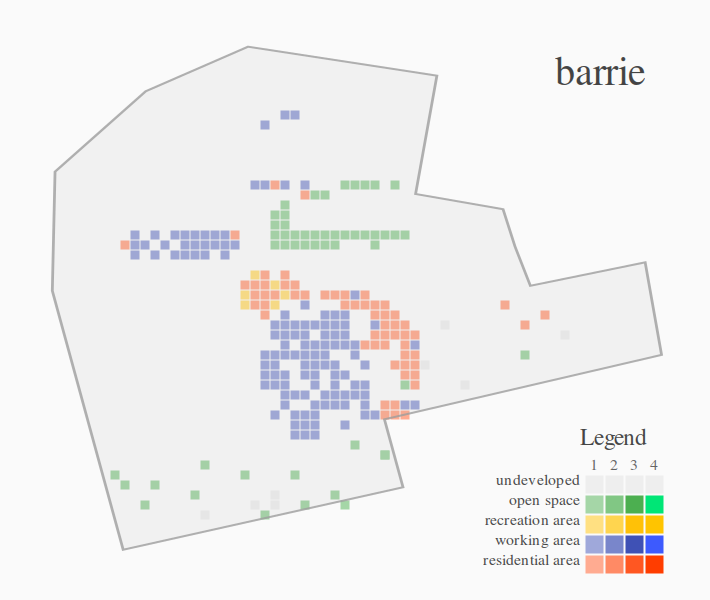
\includegraphics[width=7.5cm]{pic/barrie-patch-diff-development.png}
  \caption{Barrie development according to the government's plan}
\end{figure}

The government seems to have realized their ignorance in commercial, so the improvements concertrated in the mid S-stripe zone, the right stripe zone and at the same time improve the lake area.
It is obvious that the government still pays great attention to economic development, since 55.35\% efforts are made to working area.
The score under the government's plan is shown in table \ref{tab:barrie-score}.\\

The government of Barrie seems to take a very different approach from that of Nottingham; it emphasizes its weak points rather than becoming a tourism city.
However, the S-shape stripe zones still largely interfere with the diverse development.
It is hard to make a big change in the city's functional distribution just in a short time of 10 years.

%-------------------------------------%
%-------------------------------------%
%-------------------------------------%

\section{Growth plan based on our metric}
\emph{This section gives answers to Problem 3 \& 4.}\\

Since there are many ways to give a growth plan it's impossible for us to take all possibilities into consideration.
So we shall recommend our growth plan based on smart growth principles and certain hypothesis.

\subsection{Simplifying assumptions}
\begin{itemize}
  \item According to Pr.2, we should advocate compact building design, which means we should develop square units with low development level preferentially.
  \item According to Pr.7, we should advocate direct development towards existing communities, which means we shouldn't overdevelop unused areas. So we assume investment in unused areas or redevelopment shouldn't exceed 20\% of gross investment.
  \item According to Pr.9, in order to make decisions cost effective, we will choose the growth plan which results in maximum overall score increment.
  \item According to Pr.10, we will distribute our investment into different types of areas and adjust investment proportions.
  \item Our growth plan will use same amout of investment as the government based on previous research.
  \item We assume we will always invest the same to make a square unit development level increase one.
  \item Since government growth plans are both 10-year development plan, we will make a growth plan every 10 year and together three consecutive plans make a 30-year growth plan.
  \item We assume no square unit's development level will exceed 4.
  \item We will only redevelop open space area with 1 development(generally farmland).
\end{itemize}

\subsection{Development will function}
It's easy to see that, as for $ A_{ij} $, since its development will is negative correlated with $ d_{ij} $, $ A_{ij} $'s develop will when we add t to its development level is $$ w(i,j)=\frac{\Delta (G_m+G_b+G_h)}{t\cdot d_{ij}}=\frac{f_{r_m, k_m}^{'} (M) \cdot \Delta M + f_{r_b, k_b}^{'} (B) \cdot \Delta B + \Delta G_h}{t \cdot d_{ij}}. $$ So, we choose a square unit with the highest develop will point along with its $t$, add $t$ to its development level, and upgrade the whole map and recalculate every square unit's will point.\\

Of course we can assume the function is linear, and directly choose several square units with highest development will points, but we still choose to upgrade the map after each choice.
This actually is another type of greedy method.\\

\subsection{Nottingham's growth plan}
\begin{figure}[htb]
  \label{fig:nottingham-diff}
  \centering
  \subfigure[10 years later]{
    \label{fig:subfigure:nottingham-diff-10}
    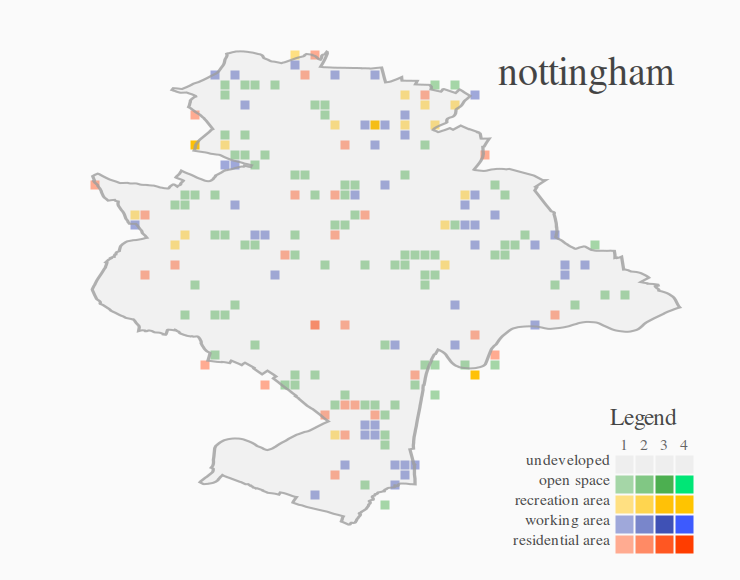
\includegraphics[width=5cm]{pic/30/nottingham-diff-10-development.png}
  }
  \subfigure[20 years later]{
    \label{fig:subfigure:nottingham-diff-20}
    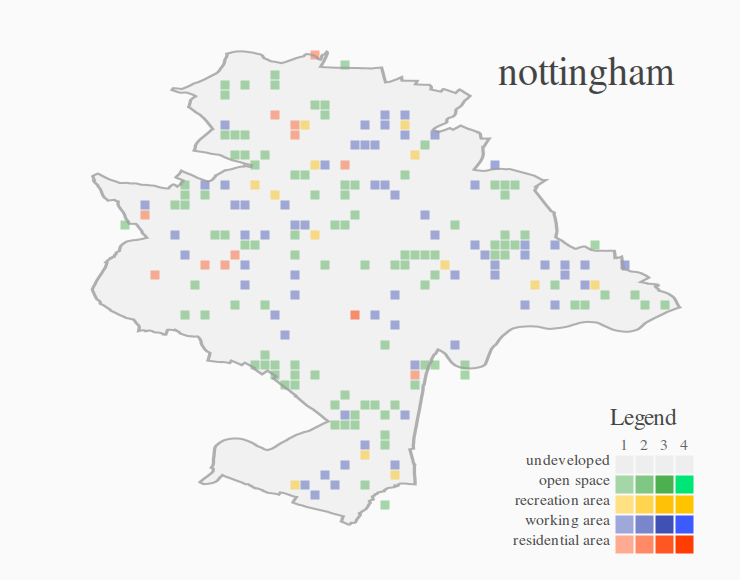
\includegraphics[width=5cm]{pic/30/nottingham-diff-20-development.png}
  }
  \subfigure[30 years later]{
    \label{fig:subfigure:nottingham-diff-30}
    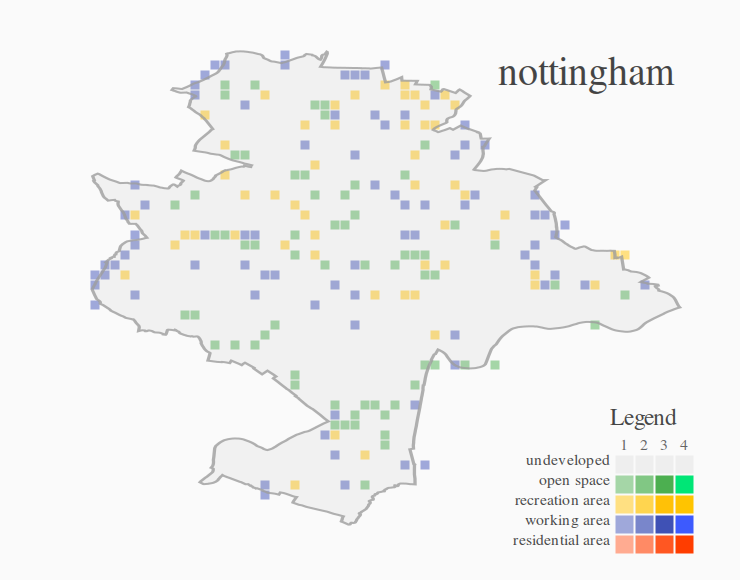
\includegraphics[width=5cm]{pic/30/nottingham-diff-30-development.png}
  }
  \caption{Nottingham's growth plan (every 10 years)}
\end{figure}
\begin{figure}[htb]
  \label{fig:nottingham-comp}
  \centering
  \subfigure[now]{
    \label{fig:subfigure:nottingham-comp-now}
    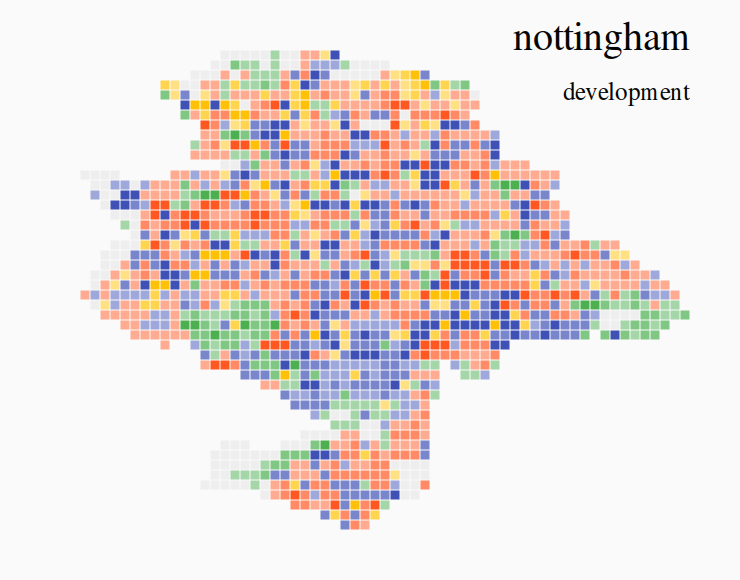
\includegraphics[width=7.5cm]{pic/nottingham-development.png}
  }
  \subfigure[30 years later]{
    \label{fig:subfigure:nottingham-comp-30}
    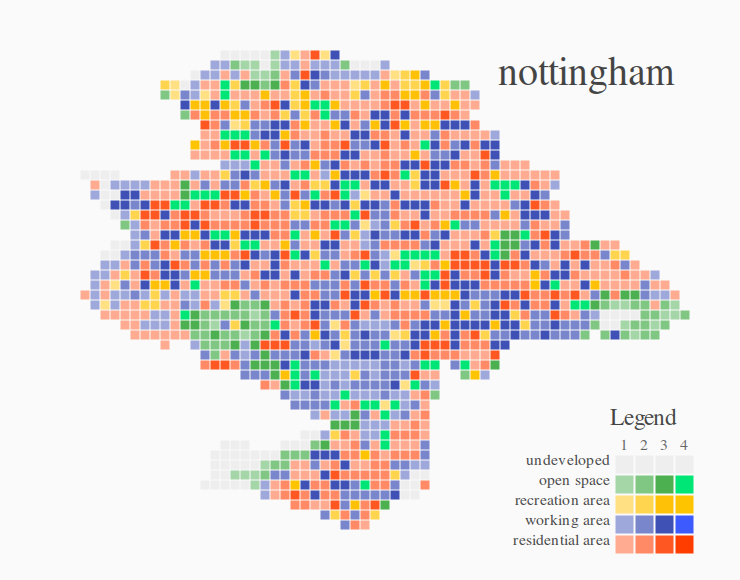
\includegraphics[width=7.5cm]{pic/30/nottingham-output-30-development.png}
  }
  \caption{A comparison in city's square units between 30 years later and present}
\end{figure}
\begin{figure}[htb]
  \label{fig:nottingham-bus-comp}
  \centering
  \subfigure[now]{
    \label{fig:subfigure:nottingham-bus-comp-now}
    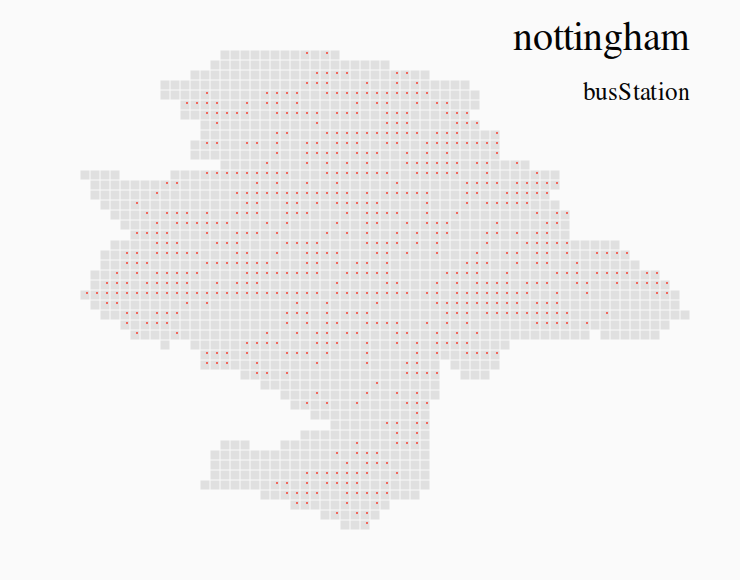
\includegraphics[width=7.5cm]{pic/nottingham-busStation.png}
  }
  \subfigure[30 years later]{
    \label{fig:subfigure:nottingham-bus-comp-30}
    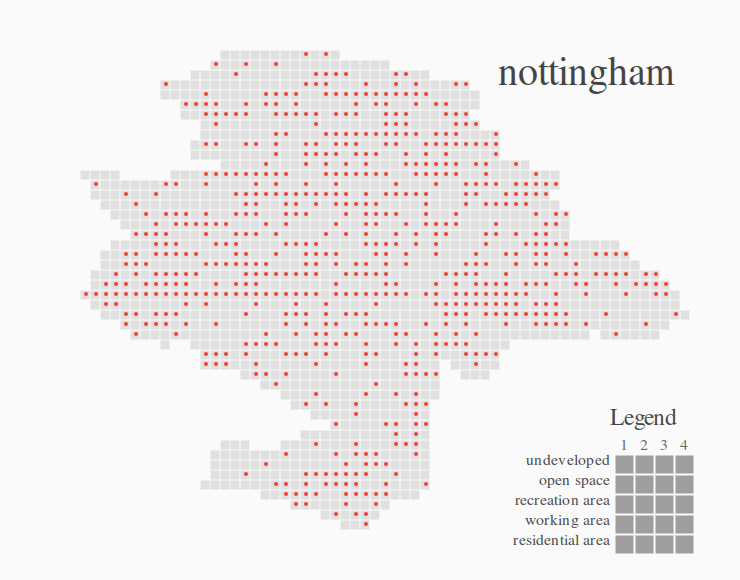
\includegraphics[width=7.5cm]{pic/30/nottingham-output-30-busStation.png}
  }
  \caption{Comparation of bus stations' distribution}
\end{figure}
Figures in \ref{fig:nottingham-diff} provide a great amount of information about how our plan can make Nottingham grow smarter.\\
\begin{table}[t]
\centering
  \begin{tabular}{c|cccc|c}
    \hline
    Item & Mix land use & Beauty & Housing & Transportation & Average \\
    \hline
    Score & 57.93 & 92.50 & 62.73 & 57.70 & 67.72 \\
    \hline
  \end{tabular}
  \caption{Nottingham Plan Score (10-Year Plan)}
  \label{tab:nottingham-model-score}
\end{table}

From data in table \ref{tab:nottingham-model-score}, we can discover that in this plan, it spends 46.39\% invesment on open space development, and relatively average investment on other three types of areas.
Housing score increases remarkably compared to government's growth plan, which can be interpreted as the reason for the plan's lack of prominent characteristic.\\

In the second 10-year growth plan, it mainly develops open spaces in the downtown (open spaces are scarce in the downtown due to its major focus on hi-tech development) and working areas in the north part of the city (residential areas and recreational areas are distributed there).\\

In the third 10-year growth plan, since the city's beauty score has increased a lot, it begins to develop working areas and recreational areas in the north part of the city. (Downtown is more developed, so it's not our priority according to Pr.2)\\

The reason for the first 10-year growth plan's irregularity is to improve low housing conditions in certain areas in the city. Next, it focuses on development in open spaces, and less focused on other areas.\\
\begin{table}[t]
\centering
  \begin{tabular}{c|ccccc}
    \hline
    Type & Residential areas & Working areas & Recreational areas & Open spaces & Undeveloped areas \\
    \hline
    Investment & 6.45\% & 23.94\% & 13.24\% & 44.14\% & 11.88\% \\
    \hline
  \end{tabular}
  \caption{Nottingham Investment Percentage (30-Year Plan)}
  \label{tab:nottingham-model-investment}
\end{table}

The 30-year growth plan is just as that in table \ref{tab:nottingham-model-investment}. It suggests that if we rank different types of areas in Nottingham from the most potential to the least potential, it would be open space,working area,recreational area,undeveloped area and residential area. Developing open spaces is to meet the need of vast natural landscape mentioned in smart growth principles, which is also the weakness of the `technology city' Nottingham. Developing working area is also Nottingham's growth need, which can be interpreted from the government's plan, which suggests that smart growth principles may not entirely correlate with a city's growth need, but definitely do not contradict with it. So in essence, smart growth principles are designed to make a city grow in a more balanced way, and meet the city's need at the same time.\\

The 30-year growth plan also have its disadvantages. Due to lack of open spaces, many open spaces downtown are developed into level 4, which is not realistic. It means in a real city growth plan, we need to adjust investment in different areas to balance the need of open space in the downtown.

\subsection{Barrie's growth plan}
\begin{figure}[htb]
  \label{fig:barrie-diff}
  \centering
  \subfigure[10 years later]{
    \label{fig:subfigure:barrie-diff-10}
    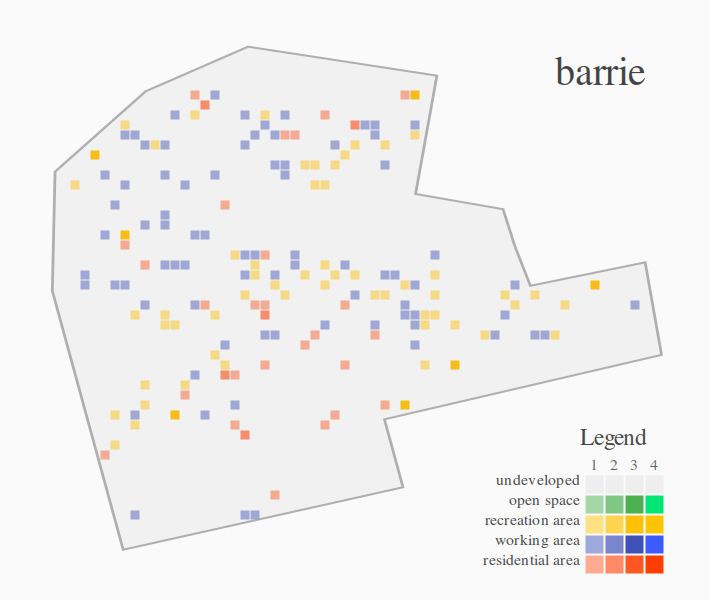
\includegraphics[width=5cm]{pic/30/barrie-diff-10-development.png}
  }
  \subfigure[20 years later]{
    \label{fig:subfigure:barrie-diff-20}
    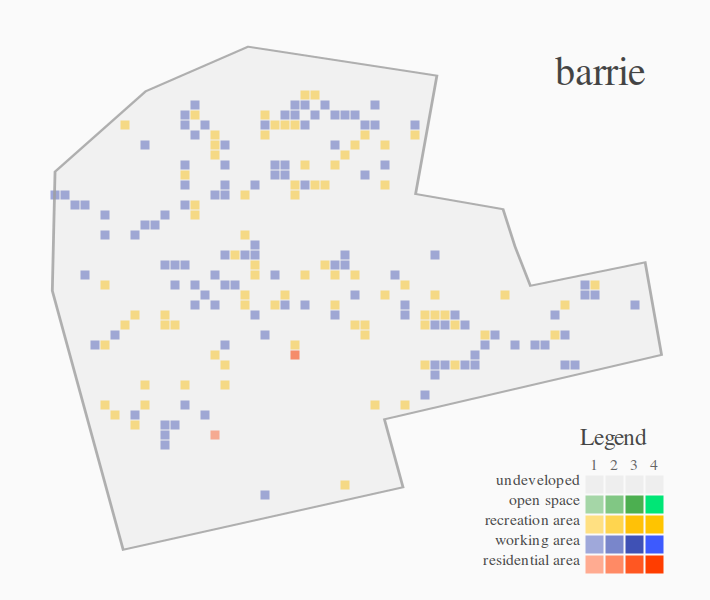
\includegraphics[width=5cm]{pic/30/barrie-diff-20-development.png}
  }
  \subfigure[30 years later]{
    \label{fig:subfigure:barrie-diff-30}
    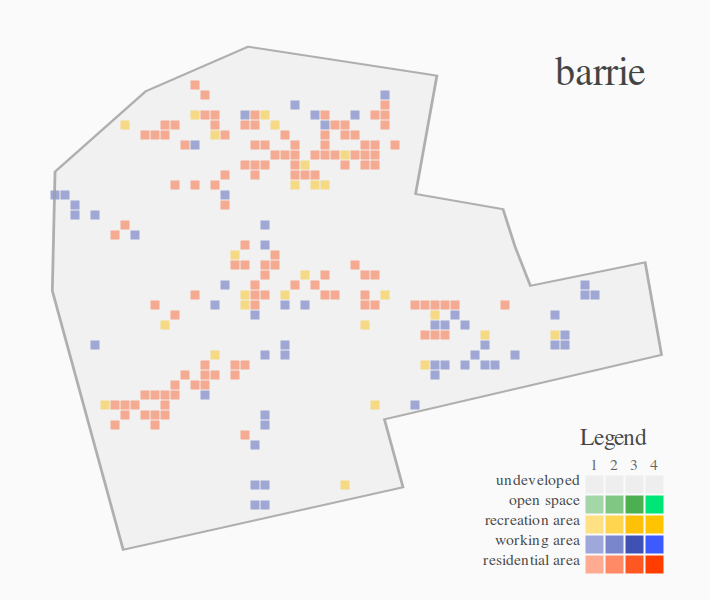
\includegraphics[width=5cm]{pic/30/barrie-diff-30-development.png}
  }
  \caption{Barrie's growth plan (every 10 years)}
\end{figure}
\begin{figure}[htb]
  \label{fig:barrie-comp}
  \centering
  \subfigure[now]{
    \label{fig:subfigure:barrie-comp-now}
    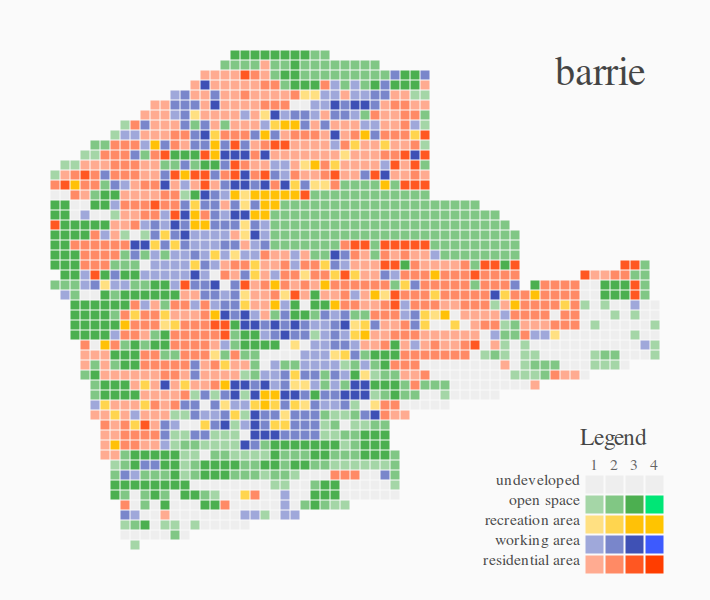
\includegraphics[width=7.5cm]{pic/barrie-development.png}
  }
  \subfigure[30 years later]{
    \label{fig:subfigure:barrie-comp-30}
    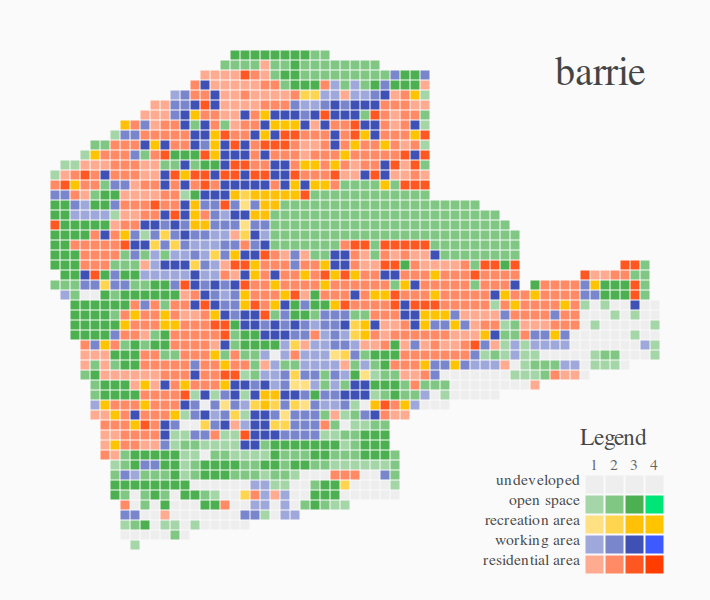
\includegraphics[width=7.5cm]{pic/30/barrie-output-30-development.png}
  }
  \caption{A comparison in city's square units between 30 years later and present}
\end{figure}
\begin{figure}[htb]
  \label{fig:barrie-bus-comp}
  \centering
  \subfigure[now]{
    \label{fig:subfigure:barrie-bus-comp-now}
    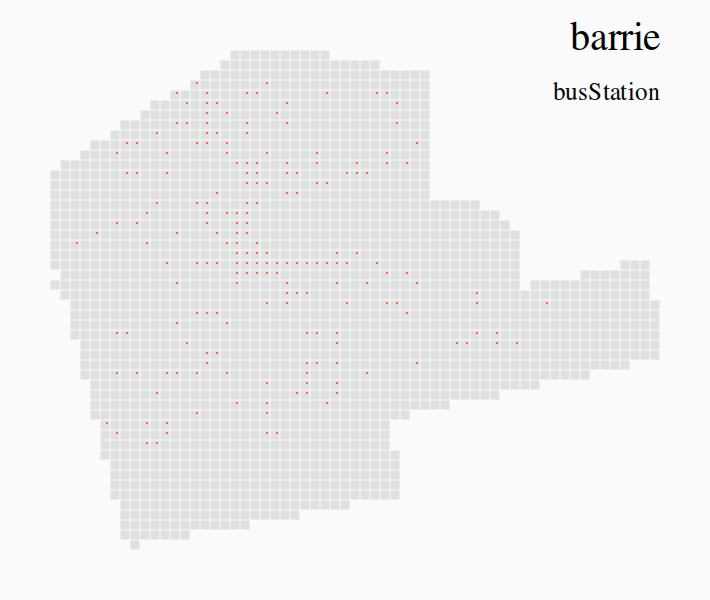
\includegraphics[width=7.5cm]{pic/barrie-busStation.png}
  }
  \subfigure[30 years later]{
    \label{fig:subfigure:barrie-bus-comp-30}
    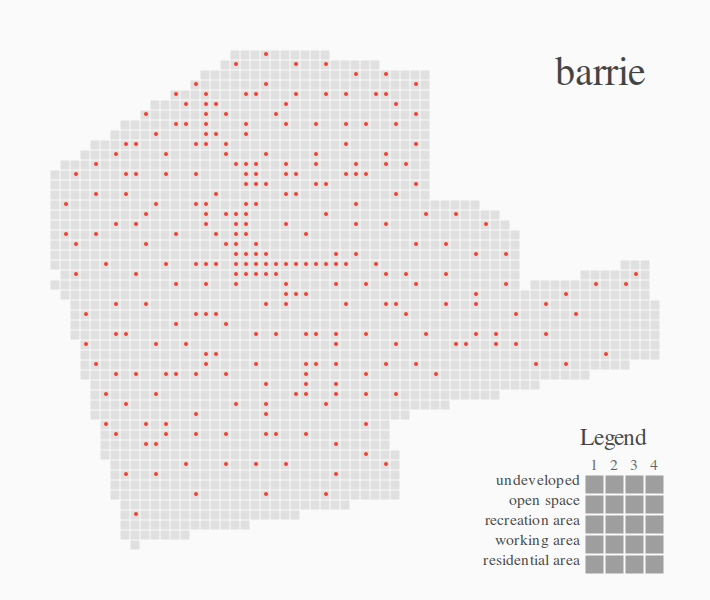
\includegraphics[width=7.5cm]{pic/30/barrie-output-30-busStation.png}
  }
  \caption{Comparation of bus stations' distribution}
\end{figure}
Figures in \ref{fig:barrie-bus-comp} provide a great amount of information about how our plan can make Nottingham grow smarter.\\
\begin{table}[t]
\centering
  \begin{tabular}{c|cccc|c}
    \hline
    Item & Mix land use & Beauty & Housing & Transportation & Average \\
    \hline
    Score & 65.88 & 92.02 & 89.42 & 66.89 & 78.55 \\
    \hline
  \end{tabular}
  \caption{Barrie Plan Score (10-Year Plan)}
  \label{tab:barrie-model-score}
\end{table}

The result of the first 10-year growth plan is listed in table \ref{tab:barrie-model-score}. It's obvious that mix-land-use and housing score increase tremendously, which is because that working areas are developed in the left side of S-shape stripe zone, where most of the square units are residential areas, and residential areas are developed in the center of S-shape stripe zone, where most of the square units are working areas. After development in this growth plan, three distinct S-shape strip zone no longer exists.\\
In the second 10-year plan, it also focuses on eliminate flat distribution of squares in the S-stripe areas in the west and east side. Because Barrie's residential areas are well-distributed, their development is not our priority.
However, in the third 10-year growth plan, in order to make up the ignorance of residential areas in the previous 10 years, it starts to develop residential areas in the middle S-stripe shape area and working areas in the south part (Most areas there are residential squares).\\
\begin{table}[t]
\centering
  \begin{tabular}{c|ccccc}
    \hline
    Type & Residential areas & Working areas & Recreational areas & Open spaces & Undeveloped areas \\
    \hline
    Investment & 24.45\% & 32.94\% & 31.41\% & 0\% & 16.30\% \\
    \hline
  \end{tabular}
  \caption{Barrie Investment Percentage (30-Year Plan)}
  \label{tab:barrie-model-investment}
\end{table}

The 30-year growth plan is listed in table \ref{tab:barrie-model-investment}. Compared to government's plan which invest 26.05\%, 55.35\% and 2.79\% respectively on residential areas, working areas and recreational areas, we can see that both plans treat residential areas similarly, but the goverment overlooks investment on recreational areas. It doesn't meet Pr.1. So if we rank different types of areas from most potential to least potential, it would be working area, recreational area, residential area, undeveloped area and open space. Since Barrie does own a lot of open spaces but lack working areas, it seems reasonable for Barrie to develop working areas first and put open space development aside.

\subsection{Summary}
Compared with Nottingham's development potential in five different types of areas, we can find that despite Barrie and Nottingham have entirely different need for open space, but any other type's development potential is quite close. Because both cities' residential parts take up most of their areas, they don't have to face high population growth pressure. So it seems less important to develop residential areas compared with working and recreational areas. Although they both develop working areas to meet their own growth need, their starting point is divergent. Nottingham develop working areas to strengthen its advantages, but Barrie is to make up for its weakness.

%-------------------------------------%
%-------------------------------------%
%-------------------------------------%

\section{Amendment}
\emph{This section gives an answer to Problem 5.}
\subsection{Simplifying assumption}
\begin{itemize}
  \item We assume that residential part holds 80\% of its total capacity at the beginning.
  \item We assume that population growth rate are identical in the three decades, and population will increase by an additional 50\% by 30 years later.
  \item We suppose that residential area has to expand at the same rate.
  \item The development of residential area is directly proportional to its population capacity.
  \item According to our simplifying assumption, city's population will reach 120\% of current population capacity 30 years later.
  \item So as we give our growth plan, every 10-year growth plan will have to face $\sqrt[3]{1.2} \approx 1.0627$ population growth, which means residential areas' total development needs to increase at least 6.27\% in every 10-year plan.
\end{itemize}

\subsection{Discussion}
We have tested how the cities develop given that the populcation changes, as is shown in the figures in \ref{fig:nottingham-amend-diff}.\\
\begin{figure}[htb]
  \label{fig:nottingham-amend-diff}
  \centering
  \subfigure[10 years later]{
    \label{fig:subfigure:nottingham-amend-diff-10}
    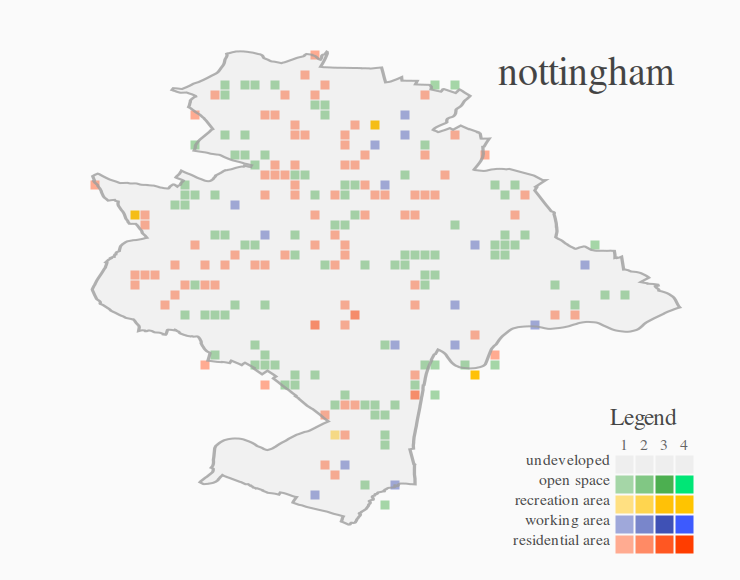
\includegraphics[width=5cm]{pic/30.5/nottingham-diff-10-development.png}
  }
  \subfigure[20 years later]{
    \label{fig:subfigure:nottingham-amend-diff-20}
    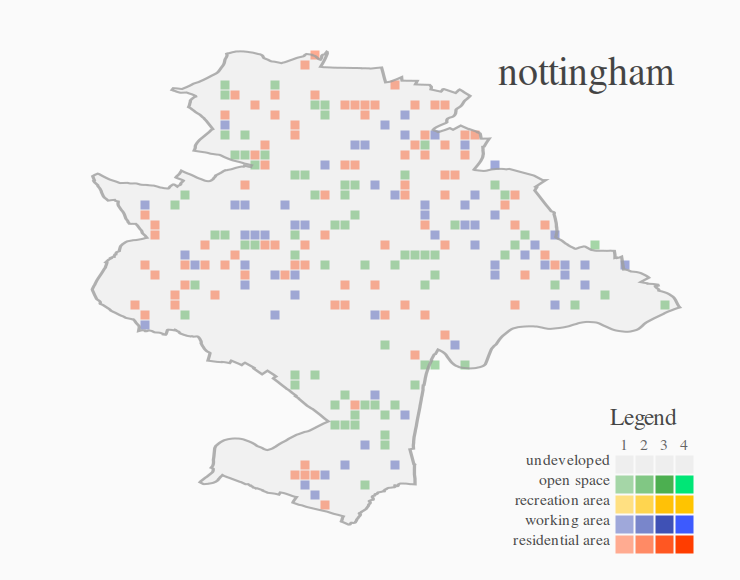
\includegraphics[width=5cm]{pic/30.5/nottingham-diff-20-development.png}
  }
  \subfigure[30 years later]{
    \label{fig:subfigure:nottingham-amend-diff-30}
    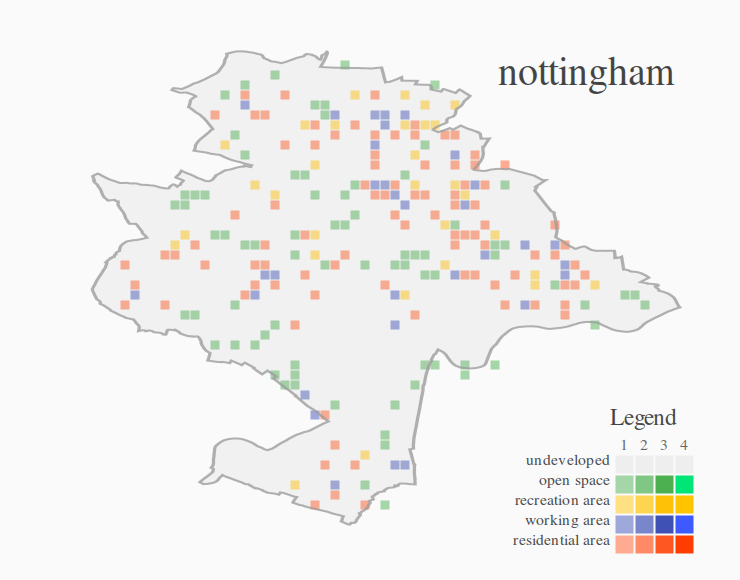
\includegraphics[width=5cm]{pic/30.5/nottingham-diff-30-development.png}
  }
  \caption{Nottingham's growth plan under new assumption (every 10 years)}
\end{figure}
\begin{figure}[htb]
  \label{fig:barrie-amend-diff}
  \centering
  \subfigure[10 years later]{
    \label{fig:subfigure:barrie-amend-diff-10}
    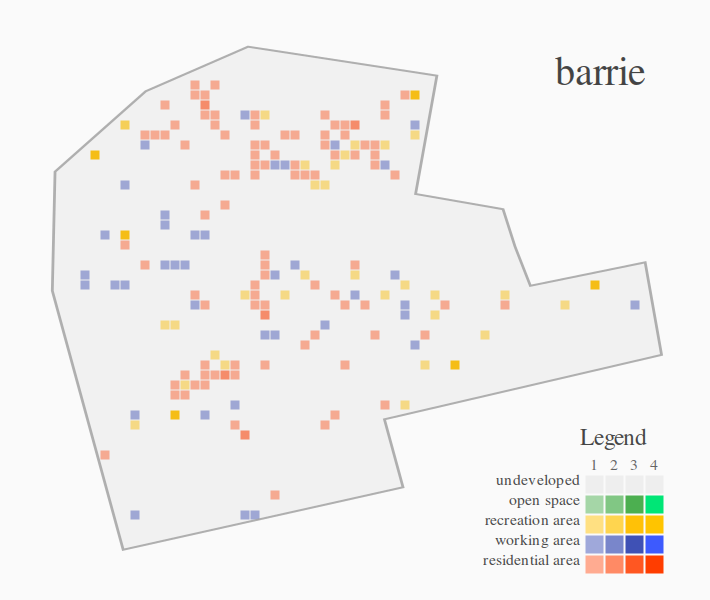
\includegraphics[width=5cm]{pic/30.5/barrie-diff-10-development.png}
  }
  \subfigure[20 years later]{
    \label{fig:subfigure:barrie-amend-diff-20}
    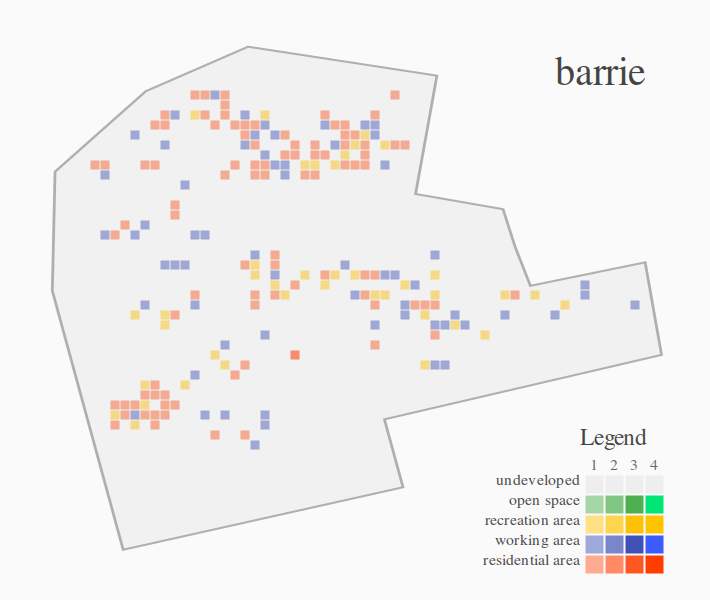
\includegraphics[width=5cm]{pic/30.5/barrie-diff-20-development.png}
  }
  \subfigure[30 years later]{
    \label{fig:subfigure:barrie-amend-diff-30}
    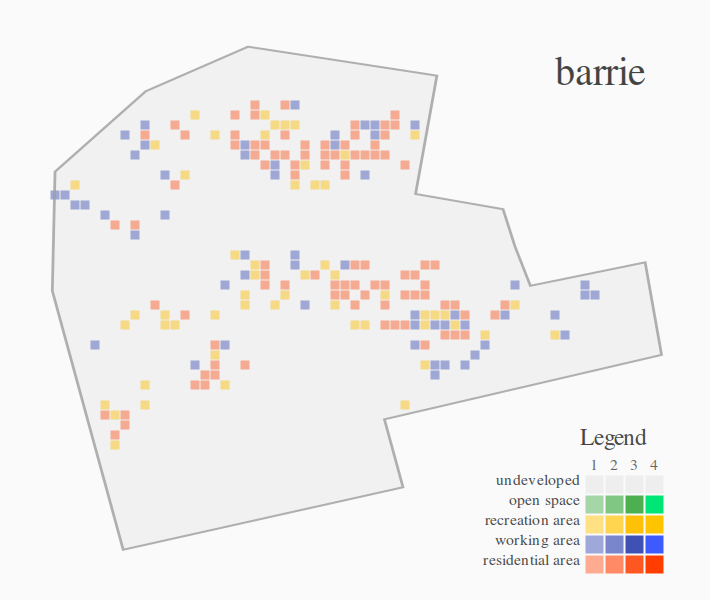
\includegraphics[width=5cm]{pic/30.5/barrie-diff-30-development.png}
  }
  \caption{Barrie's growth plan under new assumption (every 10 years)}
\end{figure}

Nottingham's growth plan under population pressure encounters the same growth problems as before. Even worse, since the downtown's development is high enough, according to Pr.2 the plan won't develop downtown first. But forced by population pressure, Nottingham has to develop residential areas in peripheral areas. Therefore, open spaces are not well-developed because of residential areas' restriction, which directly leads to lack of development in open spaces around the downtown and makes downtown's development lag behind.\\

In Barrie's 30-year growth plan, due to even heavier population pressure, more residential areas need to be developed. But affected by the lake in the northeastern part, residential areas are divided into two horizonal stripe. Other types' development are also gradually form two stripes. However, the city's mix land use is more rational compared to former plan. The potential problem that overdeveloping lakeside areas results in water contamination cannot be ignored.\\

As we can see, due to limited investment in city's square units, when population pressure increases, the city's square units change may largely depend on how residential areas are distributed. Especially in Nottingham's case, the original downtown part, including Biocity and Boots, will move towards north. Several hi-tech industries in the former downtown areas may not be well-developed, and the whole city's economic pattern may completely change.

\section{Summary}
We use partition theory in Athens Charter \cite{conf:The-Athens-Charter}, define square units to 'shatter the city'. Using partition theory, we define each square units as a functional division.
Meanwhile, we summarize 10 smart growth principles as four scores closely relative to functional division: mix-land-use score, beauty score, housing score and transportation score. We use them to evaluate whether a city's development meet with smart growth principles.
Using our metric, we evaluate two specific cities, Nottingham and Barrie.\\

Nottingham focuses on technology development, but relatively ignores improve residents' living quality. At the same time, developing high-tech industries unavoidably reduces landscape and open spaces coverage areas. Nottingham has high transportation and housing score, but mix-land-use score and beauty score is not so satisfying.
The government's growth plan for Nottingham focuses on further develop high-tech industries in downtown areas. However in our plan, we suggest that the city should first develop open spaces and landscape, and develop working areas in a balanced way.\\

Barrie scores very high in beauty, due to its high forest and water coverage. But since different types of areas distribute in three S-shape stripe areas vertically, Barrie scores low in mix land use and housing choice.
The government made growth plan suggests the city should develop working areas first. However, in our plan, we argue that the city should first break the chain of S-shape stripes distribution, makes city land more mix-used, increasing Barrie's mix-land-use score and housing score.\\

After modifying the model after considering population pressure, Nottingham's downtown begins to move compared to its former downtown. Barrie, however, develop two horizonal stripe areas. So we can conclude that, smart growth principles are limited in some ways.\\

Although smart growth principles do make a city grow relatively in accordance with the city's own need, the city still tend to grow balanced in functional units due to the principles' demand for compact design.
But every city has its own charecteristics (such as hi-tech in Nottingham and tourism in Barrie). Forcing a city grow in a balanced way may not be a completely brilliant idea.
Especially after considering population pressure, the city's developing pattern will be restricted, even will give up its advantageous industries.
But this is obviously not accordant with a city's expected development.\\

Filion Pierre also mentioned that, 'It is indeed legitimate to wonder if smart growth is more than yet another planning fad critical of prevailing practices' \cite{art:pipan}.
So we think that `Smart growth principles', as a set of theories in the 90s, don't completely apply to nowadays city development. It needs certain modifications based on realistic conditions.

%-------------------------------------%
%-------------------------------------%
%-------------------------------------%

\printbibliography

%-------------------------------------%
%-------------------------------------%
%-------------------------------------%
